%!TEX root = ../thesis.tex
% This paragraph covered a lot of ground, but I was a bit lost since each sentence tried to cover too many different approaches. Is there an implied structure? E.g. first software-static, then software-video, then physical tasks? Id’ have expected some more basic references early on that for example show that people don’t read software documentation and instead look for task-centered learning materials. There’s also a difference between related work that investigates what good instruction formats are, and systems work that introduces new tools to create such formats.

\chapter{Background}
\label{chapter_background}

This dissertation proposes computational methods to create interactive tutorials for software applications and physical tasks. To ground our work in existing practices and principles, in this chapter, I define the terminology commonly used by tutorial researchers and online community (Section \ref{background_terms}).
%
I survey research studies and literature about the motivations of people creating, sharing, and consuming tutorials (Section \ref{background_why}) and a common creation process (Section \ref{background_creation}).
%
These insights are obtained from the following resources:
\begin{itemize}
  \itemsep -2pt
  \item Formative studies from my research projects \cite{Chi:2012:MAG:2380116.2380130,Chi:2014:DRS:2556288.2557254,Chi:2013:DGC:2501988.2502052}.
  \item Guidelines for creating instructions \cite{InstructableHowTo,wikiHowHowTo}.
  \item An online survey of 2600 individuals across DIY communities \cite{Kuznetsov:2010:REA:1868914.1868950}.
  \item Interviews of tutorial authorship and learning \cite{Torrey:2007he,Torrey:2009fc,Wakkary:2015:TAH:2702123.2702550}.
\end{itemize}

% -------------------------------------------

\section{Instructions: Terminology}
\label{background_terms}

A \keyword{tutorial}, or a \keyword{how-to}, is a representation that transfers domain-specific \keyword{know-how} by describing a set of \keyword{instructions} on how to accomplish a specific task. Torrey \ea{} defined \cite{Torrey:2007he}:
\begin{quote}
\iquote{A How-To refers to online content that describes how something is done.}
\end{quote}
%
The title of a tutorial describes the goal of the task, such as ``How to retouch photos with Photoshop'' or ``Create holiday photo cards.''
%
Instructions have been widely created for various domains, including:

\begin{itemize}
  \itemsep -2pt
  \item Software applications, such as creating a motion blur effect of an image or creating a pie chart from a spreadsheet using specific software,
  \item Do-It-Yourself (DIY) projects, such as wrapping a gift box, assembling a piece of furniture, or building electronics with Arduino,
  \item Everyday activities, such as cooking or operating a vacuum machine, and
  \item Sports, such as making a dance move or swing a golf club.
\end{itemize}

Figure~\ref{fig:background_activities} shows example activities of these domains from online tutorials.
\\

% A task-centric tutorial often involves domain-specific \keyword{know-how}, knowledge that is required to perform a task.
%
Instructional content is commonly structured as a list of \keyword{steps} or \keyword{subtasks} in a linear, \keyword{step-by-step} order.
%
It is important to include essential information required to complete a task, including materials, tools, preparation, expected outcome, and tips.
%
In some domains, instructions have been derived into specific formats. For example, cooking recipes contain not only actions but also food ingredients and required amounts.
% The term \keyword{recipe} has been used for activities other than cooking.

Note that instructions are different from a (software) \keyword{documentation}, \keyword{manual}, or \keyword{user guide}, which is a technical document contained non-task-centric details about a particular hardware or software system. A manual does not provide step-by-step guidance to follow. To accomplish a task, one needs to identify relevant information from the documentation and reason the workflow.

\begin{figure*}[t]
  \centering
  \begin{minipage}{\textwidth}
  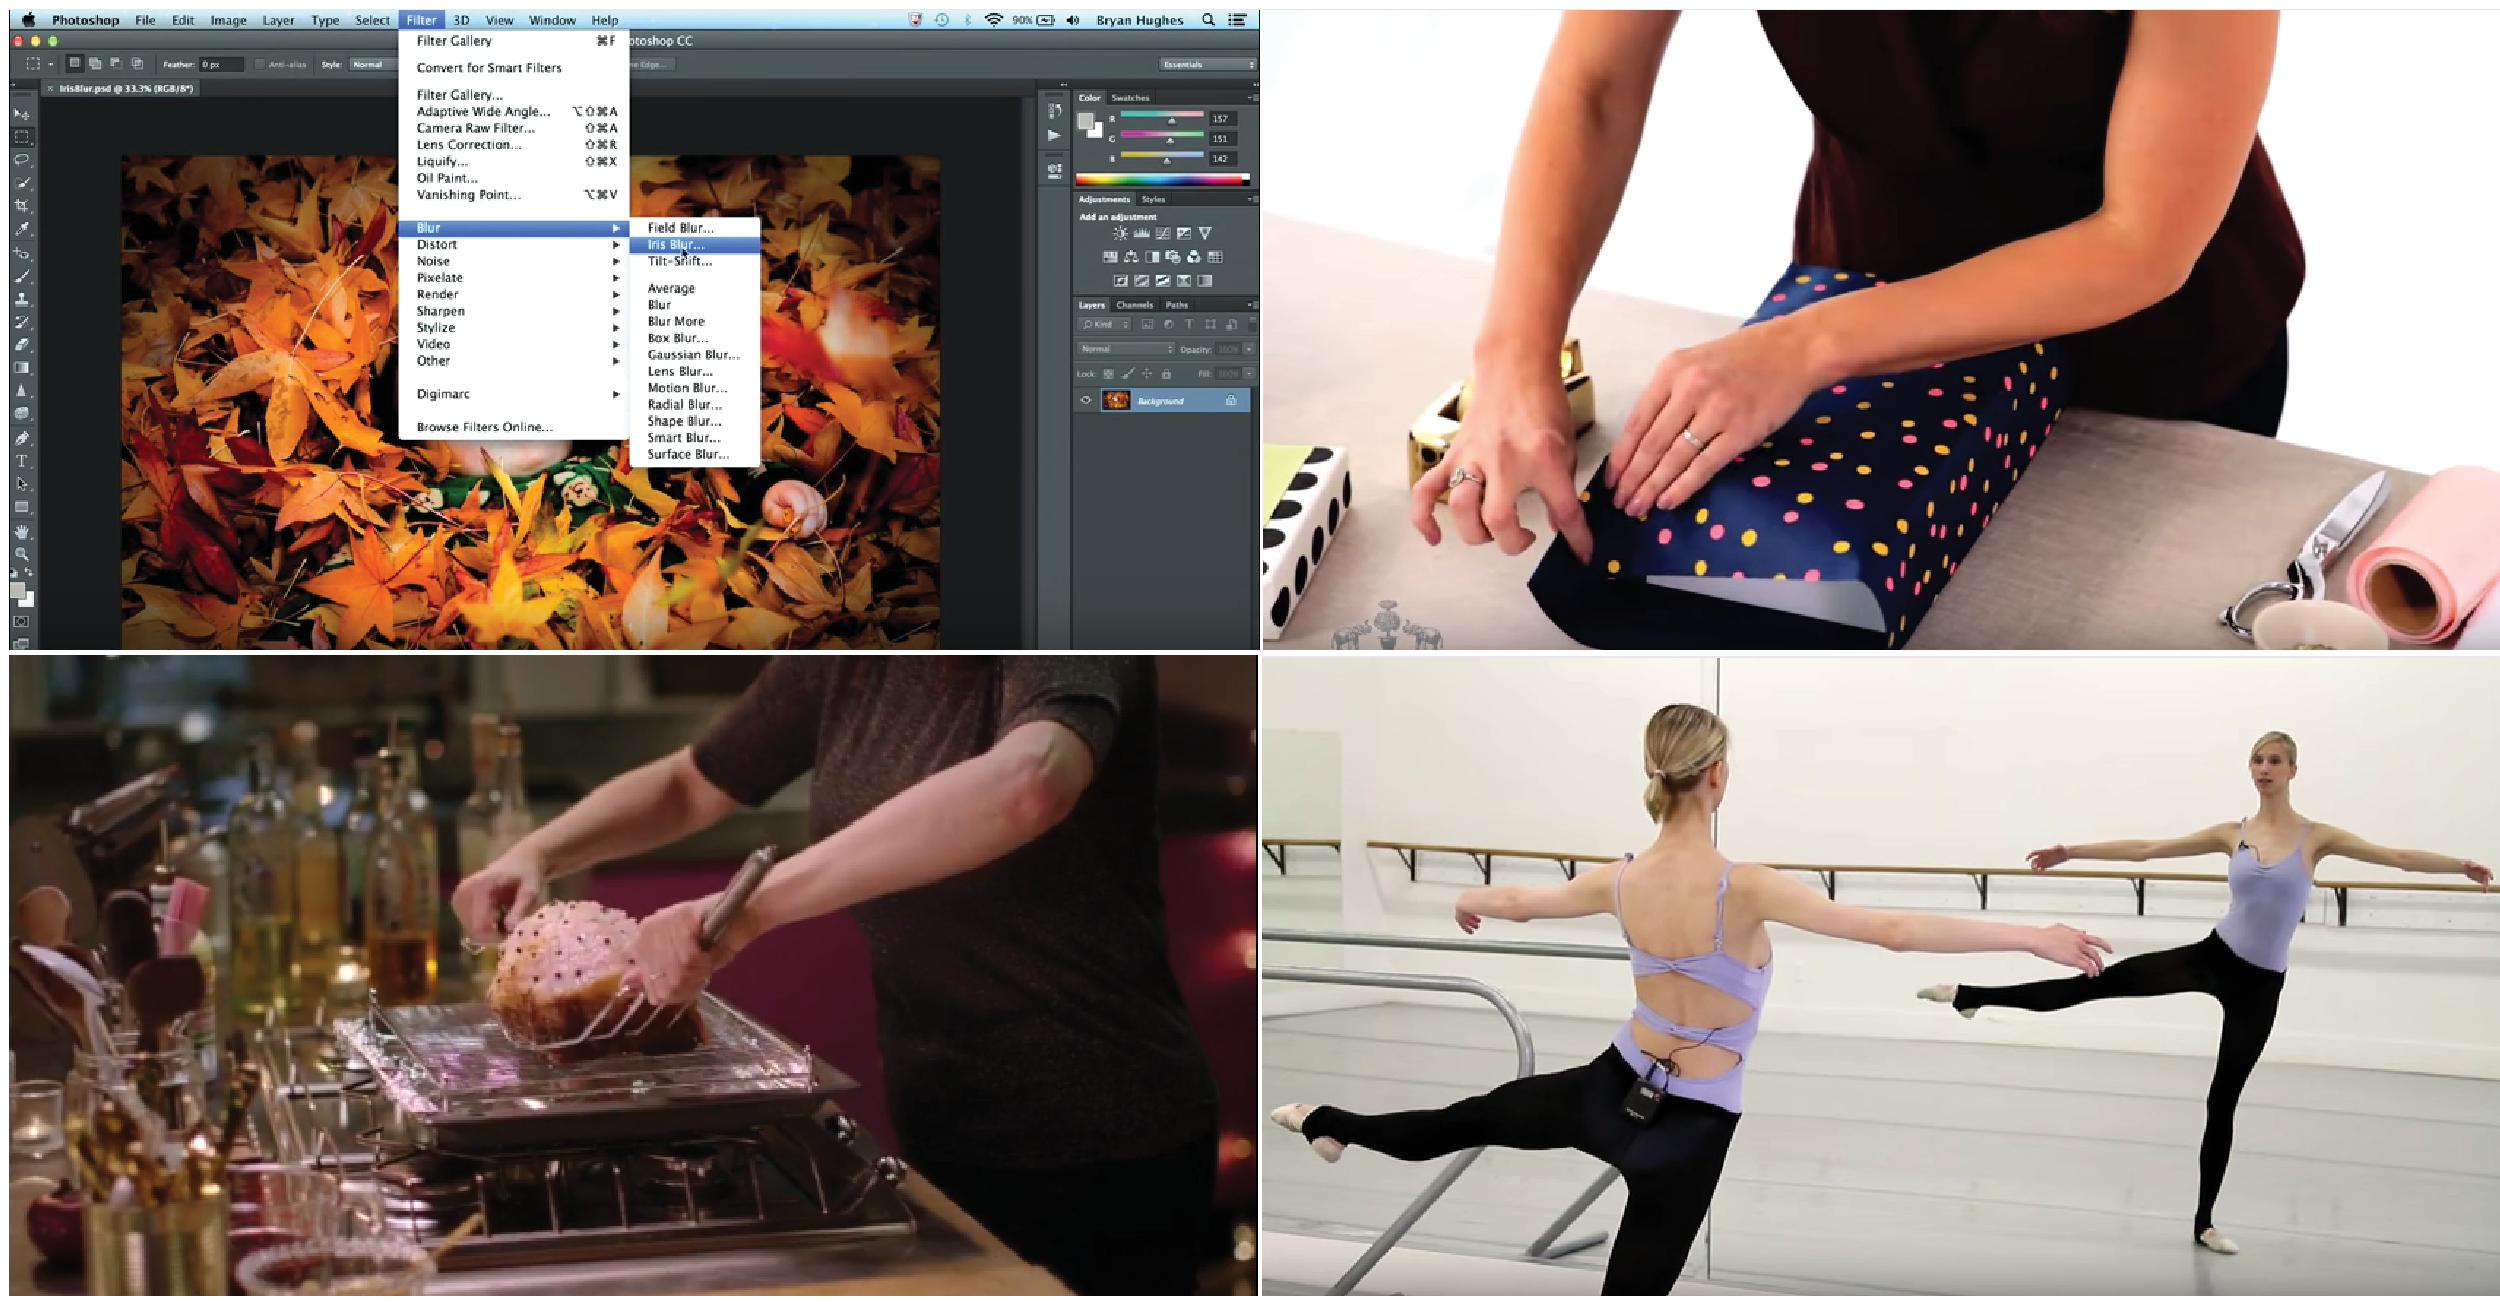
\includegraphics[width=\textwidth]{\background/fig/activities/activities}
  \caption[activities]{Example activities in tutorial domains:
  %
  a) image manipulations using a software application
  \footnote{Photoshop Playbook: Selective Focus, \url{https://youtu.be/Wh3ahxqDnyw}},
  %
  b) wrapping a gift, a DIY task
  \footnote{One Kings Lane: How to Wrap the Perfect Gift, \url{https://youtu.be/Me3ykrZobJE}},
  %
  c) cooking, an everyday activity
  \footnote{Slow-cooked black treacle ham, \url{http://www.bbc.co.uk/food/recipes/slow-cooked_black_21152}}, and
  %
  d) ballet dancing in sports
  \footnote{Ballet 101: How to Do the Fouette in Ballet Dancing, \url{https://youtu.be/DzqQNlaahjs}}.
  }
  \label{fig:background_activities}
  \end{minipage}
\end{figure*}

% -------------------

Instructions can be shown in different forms. There are two main forms of visual tutorials (see Figure~\ref{fig:background_formats}):
\begin{itemize}
  \itemsep -2pt
  \item \keyword{Static tutorials}, which use text and figures to describe the set of operations required to accomplish a task. Such format is presented as a written document with a step-by-step list, while each step includes text description and/or an image or abstract illustration to describe the subtask. It can possible be combined into a \keyword{diagram} that shows the step procedure. Static tutorials are suitable for printing and are easy to scan because they show all instructions.
  \item \keyword{Video tutorials}, which are edited or raw videos of the tutorial author performing the task. Examples include screen recordings of a software application or a camera recording of a DIY task. Videos are effective to present the work in action, especially when the activities are hard to be described in text.
\end{itemize}

\begin{figure*}[th!]
  \centering
  \begin{minipage}{\textwidth}
  \includegraphics[width=\textwidth]{\background/fig/formats/formats}
  \caption[formats]{Major tutorial forms:
  %
  a) Step-by-step static tutorials show a list of steps, each with text and figure(s) that describe a subtask
  \footnote{Combine photos on the go, \url{https://helpx.adobe.com/mobile-apps/how-to/combine-photos-photoshop-mix.html}}, and
  %
  b) video tutorials show an author performing the task, which can be reviewed via a video player
  \footnote{Change the color of an object, \url{https://helpx.adobe.com/photoshop/how-to/change-color-object-photoshop.html}}.
  }
  \label{fig:background_formats}
  \end{minipage}
\end{figure*}

% -------------------

\subsection{Creating Instructions}
Instructions are created by one or more \keyword{authors} who document the process of completing a task and refine the material to a final deliverable.
%
Since the process often involves innovations and creations of the tasks of interests, authors can also be referred as \keyword{creators}, \keyword{makers}, or \keyword{hobbyists}.
%
Instructional authors are often the \keyword{professionals} or \keyword{experts} in the domains of their work. However, in tutorial production, they might be \keyword{amateurs} or \keyword{novices} who are not familiar with software tools to refine the documented material.

Throughout this dissertation, we call the process of author completing a task as a \keyword{demonstration} or a \keyword{performance}. Authors can therefore be as \keyword{demonstrators} or \keyword{presenters}.
%
In software, the demonstration process can be referred as a system \keyword{walkthrough}. Section \ref{background_creation} will discuss the \keyword{production} process of instructions.

% -------------------

\subsection{Consuming Instructions}
We define people who review instructional content as \keyword{viewers} or \keyword{learners}. Viewers may also be \keyword{followers} if they choose to follow the instructions in action to achieve the same or similar tasks.
%
Studies have shown that learners with different learning needs and habits have various preference on the tutorial formats. In Chapter \ref{chapter_mixt}, I'll examine these differences and propose a new instructional format.

% lecturer and online tutoring: involve more feedback collection and response to learners, beyond the scope of this paper

% -------------------------------------------

\section{Why Instructions?}
\label{background_why}

The research community has been investigating the motivations behind tutorial authors creating how-to videos and written instructions.
%
In early 90s, researchers studied users who formed online communities to collaboratively customize CAD systems \cite{Gantt:1992:GGP:142750.142767}. ``Local experts'' were found to play the key role within user groups. They provided supports to CAD system users of various levels of expertise by sharing customized environments and programmatic extensions. These experienced users were not professional programmers, but they were motivated by the frustrations of following manuals with existing software.

The rise of maker movement from the 2000s introduced massive DIY project sharing via online services. Until mid-2016, Instructable has over 220,000 articles~\cite{InstructablesProjects}, and wikiHow provides 192,542 articles~\cite{wikiHowStatistics}.
%
Studies showed that one primary motivation of sharing DIY work is to demonstrate expertise ~\cite{Torrey:2007he,Kuznetsov:2010:REA:1868914.1868950}. Specifically, of the online survey that Kuznetsov and Paulos conducted in 2010 ~\cite{Kuznetsov:2010:REA:1868914.1868950}, 97\% of their 2608 respondents shared and contributed to projects to ``Express myself/be creative.'' Published tutorials serve as a way to broadcast skill and as an online portfolio.
%
Authors may derive revenue through advertising or referrals~\cite{Lafreniere:2012tl}, which was similar to how local, non-professional experts gained formal supports in CAD communities that Gantt \ea{} found \cite{Gantt:1992:GGP:142750.142767}.

Viewers, on the other hand, typically seek technical explanations, but are also searching for inspiration~\cite{Torrey:2009fc} and looking for validation of existing skills~\cite{Lafreniere:2012tl}.
%
It was shown that people prefer web-based tutorials over manual as they provide ``an immediate, specific goal to accomplish'' and can help learners ``shadow and experience an expert's work practices'' \cite{BenLafreniere:2013ux}.

While these studies present motivations on broadcasting and consuming instructions, creating ready-to-publish content can be time-consuming ~\cite{Kuznetsov:2010:REA:1868914.1868950}. Next, I discuss current practices of a tutorial production process.

% Make channel: 1,229,404 subscribers • 253,518,445 views
% Joined Mar 22, 2006
% https://www.youtube.com/user/makemagazine
% June 19, 2016
% \cite{MakerMediaKit}

% -------------------------------------------

\section{Instruction Production Process}
\label{background_creation}

Recently, guidelines of improving tutorial authorship have been proposed \cite{Wakkary:2015:TAH:2702123.2702550}. Key findings include identifying tools and components and structuring a task into steps with a clear sequence.

\begin{quote}
\iquote{The practice of writing and sharing DIY tutorials is at the heart of the distributed production and creativity of DIY. Tutorials not only provide tutorship of particular projects, they also develop the skills and competences of those involved in DIY and, in doing so, expand the culture and practices of DIY. It is fair to say that the vitality of DIY practices relies on the effectiveness and quality of tutorials.} -- Wakkary \ea{}\cite{Wakkary:2015:TAH:2702123.2702550}
\end{quote}

Creating instructions can involve several stages, especially for activities that require more steps and time \tofix{studies here}.
%
Figure~\ref{fig:background_creation} shows a common workflow of tutorial creation:

Instructables: \cite{Tseng:2014:PVP:2598510.2598540}

\subsection{Planning}
Authors make a

\subsection{Capturing}
Mutlimedia material is often used to document a process:
\begin{itemize}
  \itemsep -2pt
  \item Static photographs capture specific moments in a procedure.
  \item Video footages record a computer screencast or a scene of a demonstration.
  \item Audio recordings preserve the sound of activities or author narration.
  \item Other domain-specific content (e.g., code, board layouts, 3D models, and sketches) or resources (e.g., books or URLs to other material) often enrich the instructions.
\end{itemize}

\subsection{Editing}
Once ... to make it in a readable or viewable form

\subsection{Reviewing}

\subsection{Releasing/Sharing}
Finally, authors may release the refined content and share the deliverable with others. Common media or platforms include: personal blogs, content sharing sites (e.g., YouTube, Instructables), forums, emails, or private networks.

Some tutorial creators, especially professionals, may work as a team with multiple role players in a production process, while some work individually. The time required to create a tutorial may vary from a few minutes to weeks.
% , depending on the stages involved and the content.

\begin{figure*}[t]
  \centering
  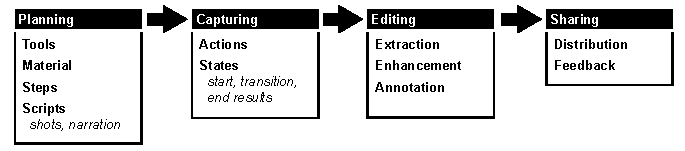
\includegraphics[width=\textwidth]{\background/fig/creation_process}
  \caption{A common workflow of tutorial creation. \tofix{update the fig}}
  \label{fig:background_creation}
\end{figure*}

These studies and observations suggest that tutorials have a larger variety of purposes and uses than merely communicating technical content.
%
In my dissertation, I strive to make authoring of instructions more accessible to amateurs while maintaining opportunities for adding individual style through control over editing effects.
%
Next, I survey prior work on computational methods of supporting authoring and following instructions.
